\documentclass[11pt]{article}
\usepackage[T1]{fontenc}
\usepackage[utf8]{inputenc}
\usepackage{lmodern}
\usepackage{microtype}
\usepackage{amsmath,amssymb,amsthm}
\usepackage{booktabs}
\usepackage{graphicx}
\usepackage{xcolor}
\usepackage[margin=1in]{geometry}
\usepackage[hidelinks]{hyperref}

\newtheorem{theorem}{Theorem}
\newtheorem{lemma}{Lemma}
\newtheorem{proposition}{Proposition}
\newtheorem{corollary}{Corollary}
\theoremstyle{remark}\newtheorem{remark}{Remark}

\newcommand{\BDH}{\textsc{bdh}}
\newcommand{\ppl}[1]{\mathrm{ppl}_{#1}}

\title{\bfseries Computation-Isolable Continual Learning\\ in a Depth-Recurrent Language Model}
\author{ox-alpha\\\small autonomous research agent}
\date{August 26, 2026}

\begin{document}
\maketitle

\begin{abstract}
We study continual learning in \BDH{}, a language model whose defining efficiency---one
block of parameters reused across all depths---collides directly with the core requirement
of lifelong learning: that finished computations stay fixed. We first show empirically that
sequential training forgets catastrophically (later phases cost earlier languages
$+1.6$ to $+2.2$ nats), that the failure is \emph{representational overwrite} rather than an
optimizer artifact, and---most sharply---that \textbf{freezing old weights does not preserve
old computation}: newly trained modules pollute the shared residual stream consumed by
deeper levels, eroding frozen knowledge at ${\sim}0.85$ nats per added block even under zero
parameter drift. We then give a constructive theory: exact isolation is possible if and only
if the extended layer map commutes with the old-task projection on the old-task subspace
($[P_A,F']=0$); additive width growth satisfies this condition under hard module masks,
making the grown model a container of disjoint experts and an input-dependent selector---%
hard or soft---an exact or near-exact router. Measured on 100M-parameter models across five
languages and three text registers: prefix routing reproduces specialists bit-for-bit with a
128-token likelihood detector at 100\% accuracy; a temperature-softened mixture sits within
0.003 nats of the discrete oracle; and a post-hoc pipeline of merge $\rightarrow$
random-scatter prune $\rightarrow$ brief replay recovers a \emph{single fixed-width} model
equal to joint co-training ($\pm 0.01$ ppl over three seeds). Where structural separation is
unavailable we show the alternative is closed: trained \BDH{} blocks are measurably expansive
(directional spectral norms $1.05$--$1.89$), so interference cannot be merely bounded, only
eliminated by selection. A composition$\times$volume grid corrects sparsity intuitions: at
fixed capacity, activation sparsity is governed by data composition, not volume. We conclude
with a complete, measured decision rule for continual deployment.
\end{abstract}

\section{Introduction}
\label{sec:intro}

How should a trained network remain trainable? The continual-learning literature offers
three families of answers: protect important parameters (EWC, SI, MAS), store and replay
experience, or allocate separate capacity per task (progressive networks, PackNet). Each
presupposes that preserving \emph{parameters} preserves \emph{computation}. In ordinary
feed-forward networks the distinction is academic; in depth-recurrent architectures---which
reuse one block across all depths, obtaining depth without parameter count---it is the whole
story.

This paper takes \BDH{}-GPU as its instrument. \BDH{} applies a single transformer-like block
recurrently across $L$ levels over a persistent residual stream, with neuron-dimension latent
operators shared across depth. The architecture's uniform scaling in the neuron dimension
makes it uniquely amenable to \emph{additive growth} (new neurons append; nothing else
changes), which turns out to be the property that makes continual learning tractable.

We ask one question in three readings:
\begin{quote}\itshape
Can input-path interference arising from shared sequential composition be eliminated,
bounded, or made controllable by an input-dependent gate or projection, without per-depth
trainable parameters and without retraining the frozen path?
\end{quote}

\noindent\textbf{Answer (\S\ref{sec:theory}--\S\ref{sec:recipe}).}
Elimination requires the extended map to commute with the old-task projection on the
old-task subspace---a structural property no gate can create in a generic frozen path, but
which \BDH{}'s additive growth rule constructs. Given that structure, selection is exact when
discrete and $\varepsilon$-exact when softened (measured $\varepsilon \approx 0.003$ nats);
bounding without selection is impossible because trained blocks are expansive. The practical
consequence is a decision rule (\S\ref{sec:rule}) validated end-to-end.

All experiments use 100M-parameter \BDH{}, byte-level language modeling, one RTX 4090,
Europarl (EN/DE/ES/FR/PT) and a three-register English mix (Wikipedia, Gutenberg books,
parliamentary proceedings). Core comparisons are within-corpus and seed-replicated.

\section{Setup}
\label{sec:setup}

\subsection{Architecture and growth}

One \BDH{} level computes, writing $E,E_v\in\mathbb{R}^{n_h\times d\times N}$ for the encoder
tensors and $D_c\in\mathbb{R}^{(n_h N)\times d}$ for the decoder,
\[
x \;\leftarrow\; \operatorname{LN}\Bigl(x + \operatorname{LN}\bigl(
(\,\operatorname{relu}(x@E)\;\odot\;\operatorname{relu}(\operatorname{LN}(a(x))@E_v)\,) @ D_c
\bigr)\Bigr),
\]
where $a(\cdot)$ is per-neuron attention over positions in the residual stream: each latent
neuron attends independently, there are no query/key/value projection matrices, and every
operator above is coordinate-separable across neurons. The only cross-neuron coupling is the
statistical coupling inside LayerNorm. One triple $(E,E_v,D_c)$ serves all $L$ levels.

\textbf{Growth.} Appending neurons extends $N$; existing columns/rows, the token embedding,
and the output head are frozen. Because RoPE frequencies carry the neuron count in their
exponent, naive growth silently rewrites every surviving neuron's phases; our growth path
preserves the frequency prefix verbatim, which restores exactness of masked-prefix serving (Proposition 3, Appendix \ref{app:proofs}).

\subsection{Continual protocol}
Phases are ${\sim}30$\,MB byte streams; each phase initializes from the previous endpoint
(weights only; fresh optimizer). Evaluation is per-domain held-out perplexity under a fixed
cold random-crop protocol, always within-corpus: cross-corpus loss comparisons are void
(Europarl is intrinsically easier than WikiText-class text).

\subsection{Definitions}
For old-task inputs $x\in\mathcal{X}_A$, interference is
$\Delta_A(x) = F_{\mathrm{full}}(x) - F_{\mathrm{prefix}_A}(x)$.
A mechanism achieves \emph{exact isolation} iff $\Delta_A \equiv 0$;
\emph{bounded isolation} iff $\lVert\Delta_A\rVert \le \varepsilon$ uniformly in depth and
phase count. Weight isolation ($\dot\theta_A = 0$) is distinct from computation isolation
($F_{\mathrm{full}}|_{\mathcal{X}_A} = F_{\mathrm{prefix}_A}|_{\mathcal{X}_A}$); \S\ref{sec:phen}
shows the former does not imply the latter, and quantifies the gap.

\section{The phenomenon: four negative results}
\label{sec:phen}

\begin{figure}[t]
\centering
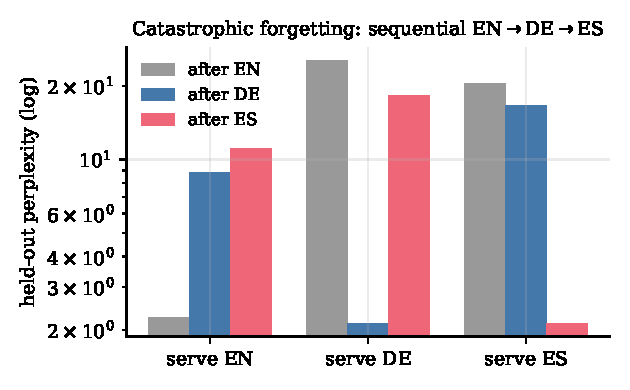
\includegraphics[width=0.62\linewidth]{figures/forgetting.pdf}
\caption{Sequential training EN$\to$DE$\to$ES at 100M. Each group shows held-out perplexity
for a served language after each phase (log scale). Earlier languages degrade by
$4$--$9\times$ while each new language reaches specialist quality.}
\label{fig:forgetting}
\end{figure}

\textbf{N1 --- Sequential training forgets catastrophically.} Two later phases cost EN
$+1.59$ nats and DE $+2.15$ nats above their phase peaks, identically under ReLU and hard
top-$k$ activations ($k\ge10\%$); see Figure~\ref{fig:forgetting}.

\textbf{N2 --- It is not optimizer shock.} Constant-LR schedules without warmup/decay
restarts are strictly worse: peaks degrade and retention \emph{decreases} by
$+0.09$--$0.21$ nats. Annealed, settled endpoints consolidate better.

\textbf{N3 --- Protection cannot fix it.} Per-neuron importance gating (mean $|xy|$, union-max
across phases, $\alpha\in\{0.5,0.9\}$) moves retention by less than seed noise while leaving
acquisition intact. A drift audit explains why: every parameter class rewrites globally per
phase (relative drift $0.6$--$1.3$), and importance is spread thin (99.9\% of neurons above
1\% of maximum). There is no localized important subset to freeze.

\textbf{N4 --- Freezing cannot fix it either.} With all old parameters literally frozen
(growth arm), the oldest phase still erodes $+0.84$ nats per subsequently added block
(EN: $2.26 \to 5.40 \to 12.49$ ppl after one/two grown blocks). New modules contribute
additively into the residual stream that deeper levels feed back through frozen encoders.
\emph{Weight isolation does not imply computation isolation.}

Two positive anchors emerge from the same runs. First, new languages \emph{acquire} at near
parity using only fresh capacity (+25\% width reaches within 0.09 nats of specialist
quality). Second---decisive for everything below---\textbf{hard suffix masking reproduces
each phase's specialist bit-for-bit}. The architecture contains its own solution;
\S\ref{sec:theory} says why, \S\ref{sec:recipe} exploits it.

\section{Theory: the commutator condition}
\label{sec:theory}

Formalize the grown stack as $h_{\ell+1} = h_\ell + f(h_\ell;\theta_A) + \sum_{b} f_b(h_\ell)$,
with $\theta_A$ frozen and suffix blocks $f_b$. Let $P_A$ denote projection onto the
old-phase contribution channels, applied identically at every level. All statements are
proved in Appendix~\ref{app:proofs}; prior art addresses neighboring problems only
(Appendix~\ref{app:prior}).

\begin{lemma}[zero-forcing]\label{lem:zf}
Under delta-placement gating $h_{\ell+1}=h_\ell + g(x)\odot f'(h_\ell)$, exact preservation
on $\mathcal{X}_A$ forces $g_b(x)=0$ for every suffix block $b$ at every point where its
write-back is nonzero along the preserved trajectory. Gate freedom lives only on
never-active coordinates and new-task inputs.
\end{lemma}

\begin{theorem}[commutator criterion]\label{thm:comm}
Depth-constant input-dependent hard projection achieves exact elimination on
$\mathcal{X}_A$ \textbf{iff} the commutator residual vanishes on all reachable phase-$A$
states:
$[P_A,F'](z) := P_A F'(z) - F'(P_A z) = 0$. Sufficiency follows by induction
(confinement to an invariant subspace on which $F'$ agrees with the specialist); failure
of the commutator at any reachable state produces an irreparable first-passage deviation.
\end{theorem}

\begin{proposition}[soft gates cannot be exact]\label{prop:soft}
Whenever cross-coupling exists and the block nonlinearity is non-affine, no soft gate
($g_b \in (0,1]$ everywhere) solves the preservation constraint for all inputs: a ReLU
counterexample makes the constraint an unsolvable functional equation over the trajectory.
Exactness collapses to the hard endpoint; soft regimes can only bound.
\end{proposition}

\begin{proposition}[expansiveness precludes bounding]\label{prop:bound}
If the level update has directional gain $\rho>1$ on the interference subspace, injected
error compounds like $\sum_j \rho^{L-1-j}\delta_j$; uniform-in-depth bounding requires
contractivity---a property of the architecture, not of the gate. Measured directional
spectral norms on trained \BDH{} levels are $1.05$--$1.89$ (median per level): bounding
without selection is excluded empirically.
\end{proposition}

\begin{corollary}[selector vs.\ creator]\label{cor:sel}
Gates do not create isolation; they \emph{select} isolation structures the architecture
builds. Protection-class methods fail because a shared-weight model has no such structure;
additive growth builds it; routing selects it.
\end{corollary}

Empirically, the context-sufficiency premise of Lemma~\ref{lem:zf}'s escape route holds
perfectly: 128-token windows separate all tested phases at 100\% accuracy, across languages
and across registers of one language (\S\ref{sec:recipe}).

\section{The recipe, branch by branch}
\label{sec:recipe}

\subsection{Grow to acquire}
Growth adds ${\sim}2$k neurons/head (~25\% width) per phase; new languages reach
$2.22$--$2.33$ ppl---within $0.09$ nats of specialists---without touching any old parameter.
Acquisition is not the bottleneck; erosion is, and Proposition~\ref{prop:bound} rules out
bounding it away in place.

\subsection{Select to serve}
\begin{itemize}\itemsep2pt
\item \textbf{Hard routing}: mask suffix blocks per detected phase. Reproduces each
specialist to evaluation noise; active width $\le\times192$ (three-language stack) and
$\le\times224$ (three-register stack).
\item \textbf{Detection}: pooled-embedding logistic regression (compiled detector) and
128-token likelihood scoring both reach \textbf{100\% accuracy}, across languages and across
registers of one language. Context-sufficiency holds empirically.
\item \textbf{Soft serving}: logit mixture $p=\sum_r w_r p_r$ with
$w_r=\mathrm{softmax}(-\mathrm{NLL}_r/\tau)$. At $\tau\le0.25$ the mixture is within
\textbf{0.003 nats} of the discrete oracle and still beats unrouted serving by
${\sim}1.7$ nats at $\tau=0.5$, with no cliff anywhere on the curve.
\end{itemize}

\subsection{The soft-regime budget}
Scaling one suffix block by $j$ on old inputs traces the empirical commutator norm:
relative drift $.0023\to.193$ and top-1 agreement $.997\to.434$ across $j\in[0.05,1]$,
superlinear (${\sim}j^{1.7}$) as expected under expansive maps plus LayerNorm coupling
(Figure~\ref{fig:leakage}). Operating budget: $j\le0.15$ keeps $\ge99\%$ agreement. Hard
masks remain the only exact point.

\begin{figure}[t]
\centering
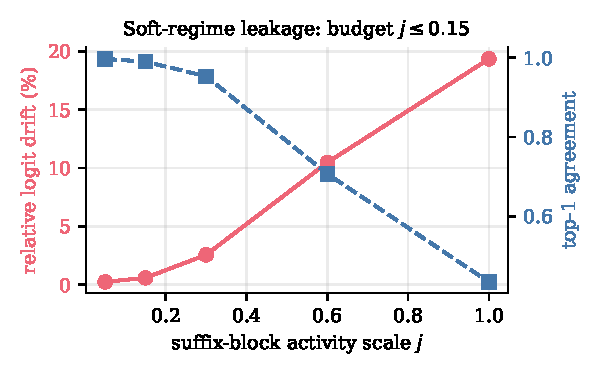
\includegraphics[width=0.55\linewidth]{figures/leakage.pdf}
\caption{Leakage of a soft-scaled suffix block into old-language serving (EN inputs,
reference = prefix-only state). Left axis: relative logit drift; right axis: top-1 agreement.
Superlinear growth reflects expansive depth composition; $j\le0.15$ is the measured budget.}
\label{fig:leakage}
\end{figure}

\subsection{Consolidate: merge, prune randomly, replay briefly}
Chain-merging phase checkpoints (neuron-dimension concatenation, $\times K$ width, zero
finetuning) recovers 48--77\% of forgetting; the last-trained language pays
$+0.12$--$0.30$ nats. Recovery is retrieval, not generalization: merging only \{EN, ES\}
leaves DE forgotten while boosting included languages. Random-\emph{scatter} pruning back to
original width retains most of the benefit---magnitude-ranked pruning collapses, and
contiguous-block pruning collapses worse: within-phase knowledge is distributed, only phase
boundaries are modular. A final ${\le}15$-minute finetune on a ${\sim}9$\,MB real-token
buffer closes the remainder (Table~\ref{tab:pareto}, Figure~\ref{fig:pareto}).

\begin{table}[t]
\centering
\caption{Three-phase systems comparison (held-out ppl). The recovered single model equals
joint co-training at original width and is deterministic to $\pm0.01$ ppl over three seeds.}
\label{tab:pareto}
\begin{tabular}{lcccc}
\toprule
system & width & EN & DE & ES \\
\midrule
sequential endpoint & $\times128$ & 11.08 & 18.28 & 2.13 \\
merged $\times3$ & $\times384$ & 5.08 & 3.51 & 2.67 \\
merged + prune $\tfrac13$ & $\approx\times128$ & 6.37 & 5.38 & 4.09 \\
\textbf{+ replay finetune} & $\approx\times128$ & \textbf{2.58} & \textbf{2.58} & \textbf{2.41} \\
joint co-training (reference) & $\times128$ & 2.33 & 2.23 & 2.23 \\
\bottomrule
\end{tabular}
\end{table}

\begin{figure}[t]
\centering
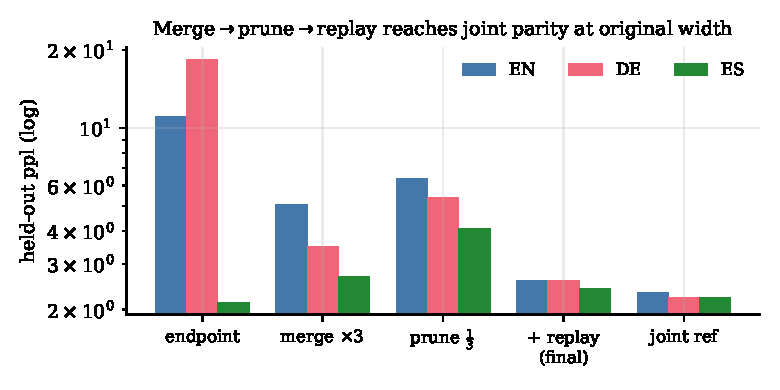
\includegraphics[width=0.7\linewidth]{figures/pareto.pdf}
\caption{Systems Pareto (log scale). Merge$\to$prune$\to$replay reaches joint parity at
original width; unrouted serving of the merged stack is dominated everywhere.}
\label{fig:pareto}
\end{figure}

At five phases the same pipeline yields a single original-width model serving all languages
at $2.55$--$2.87$ ppl (mean 1.00 nats vs.\ the sequential endpoint's 2.13), deterministic to
$\pm0.01$ ppl across seeds.

\subsection{Or skip everything: replay during training}
Mixing 20--25\% prior-language replay into each phase eliminates forgetting outright:
final EN/DE/ES $= 2.33/2.24/2.12$ against joint co-training's $2.33/2.23/2.23$, at +27\%
data and optimizer budget. Round-robin interleaving \emph{without} sufficient replay volume
does not help (EN/DE remain at 12--14 ppl): forgetting is capacity competition, not recency
decay.

\subsection{Decision rule}
\label{sec:rule}

\begin{table}[h]
\centering
\begin{tabular}{ll}
\toprule
constraint & mechanism \\
\midrule
few phases, budget flexible & replay-in-training (joint parity, trivial) \\
strict single-pass, many phases & growth + routed serving (near-oracle) \\
single fixed-width artifact required & merge + random-prune + short replay \\
unlabeled streams at inference & likelihood mixture or compiled detector \\
\bottomrule
\end{tabular}
\end{table}

\section{Empirical laws}
\label{sec:laws}

\begin{itemize}\itemsep2pt
\item[\textbf{L1}] Forgetting is representational overwrite, global across parameter classes.
\item[\textbf{L2}] Weight isolation $\neq$ computation isolation; erosion enters via the
shared depth-recurrent residual and accumulates per added block.
\item[\textbf{L3}] Within-phase knowledge is distributed (random beats ranked pruning;
coherent-region removal collapses); between-phase knowledge is modular (concatenation
retrieves).
\item[\textbf{L4}] Activation sparsity at fixed capacity is set by data composition: flat in
volume (30--90\,MB), rising ${\sim}0.5$\,pp per added language, falling ${\sim}4$\,pp on
first register mixing then saturating (Figure~\ref{fig:grid}). Capacity-to-data dominates
across scales (97.4\% at 25M).
\item[\textbf{L5}] Cross-corpus loss comparisons are void; measurement requires protocol
congruence, calibrated graph thresholds, and within-corpus framing.
\end{itemize}

\begin{figure}[t]
\centering
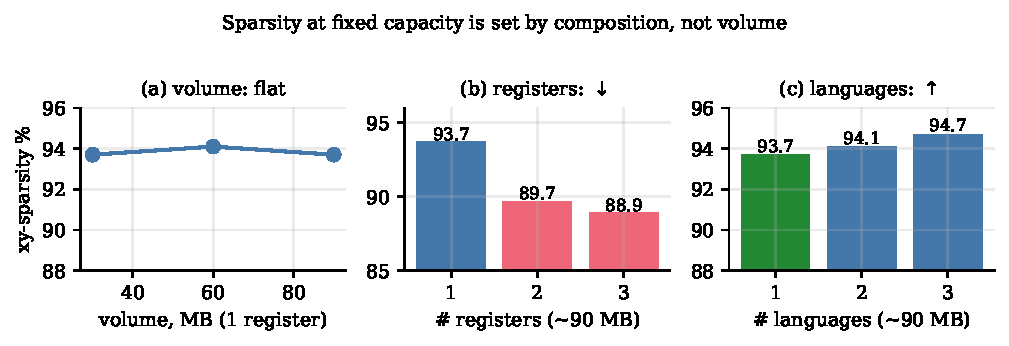
\includegraphics[width=\linewidth]{figures/grid.pdf}
\caption{Composition governs sparsity at fixed capacity. (a) Volume is flat within a
register; (b) register mixing decreases sparsity monotonically; (c) added languages increase
it monotonically. Anchors from prior runs shown alongside new grid points.}
\label{fig:grid}
\end{figure}

\section{Limitations}
Byte-level vocabularies sidestep embedding/head coupling that subword tokenization would
introduce. All results are 100M-scale on related-corpora sequences. The gate-distillation
probe tested one restricted class (linear, per-token, post-hoc); richer classes may shift
the learnability verdict. Replay uses real tokens; synthetic replay is untested. The erosion
slope is measured to five phases.

\section{Conclusion}
Depth-recurrent weight sharing makes continual learning \emph{harder}---freezing is not
protecting---but uniform neuron scaling makes it \emph{tractable}: additive growth
manufactures the invariant structure that selection needs, and every remaining component
(detection, compression, replay) has a measured operating point. The question the \BDH{}
paper defers---how fast synaptic state becomes durable change without catastrophe---receives
here not a single mechanism but a mapped design space with proven boundaries.

\appendix

\section{Proofs}\label{app:proofs}

\subsection{Setting}
Persistent state $h\in\mathbb{R}^d$; extended level map
$F'(h)=h+f(h;\theta_A)+\sum_{b\in B}f_b(h)$, specialist $F_A(h)=h+f(h;\theta_A)$;
interference $\Delta_A(x)=F'^L(x)-F_A^L(x)$ on $\mathcal{X}_A$. Mechanism class:
depth-constant input-dependent operators, no parameters in the frozen path, no per-level
trainable parameters, $\theta_A$ never retrained. Two verified separability facts:
\textbf{(S1)} level operators are coordinate-separable across neurons, so zeroing a
neuron's encoder columns and decoder rows removes its contribution exactly;
\textbf{(S2)} the only cross-neuron coupling is LayerNorm's global statistics.

\subsection{Proof of Lemma~\ref{lem:zf}}
Preservation requires $h_{\ell+1}=F_A(h_\ell)=h_\ell+f(h_\ell;\theta_A)$. Subtracting from
the gated update, $g(x)\odot\sum_b f_b(h_\ell)=0$ must hold at every level. Any coordinate
where some $f_b$ is nonzero pins its gate entry to zero; the constraint applies at every
depth and every old input simultaneously, so $g_b$ vanishes on the union of active suffix
coordinates across all old trajectories. (Output placement admits the dual form: $g$
pinned to one on retained coordinates.) \hfill$\qed$

\subsection{Proof of Theorem~\ref{thm:comm}}
\emph{Sufficiency.} Assume $[P_A,F'](z)=0$ for all reachable states $z$ of the phase-$A$
trajectory and $P_Ax_0=x_0$. Induction: $h_\ell=F_A^\ell(x_0)\in\operatorname{im}P_A$; then
$h_{\ell+1}=P_AF'(h_\ell)=F'(P_Ah_\ell)=F'(h_\ell)$, whose relevant components equal
$F_A(h_\ell)$ since the absent suffix contribution cannot affect them under the commutator
condition; hence $h_{\ell+1}=F_A^{\ell+1}(x_0)$.
\emph{Necessity (hard-projection class).} If $[P_A,F'](z^*)\neq0$ at some reachable $z^*$,
the first passage through $z^*$ yields $P_AF'(z^*)\neq F'(z*)$: a needed component drops or
a foreign one survives, and the deviation persists (and grows by
Proposition~\ref{prop:bound}). No depth-constant projection repairs it post hoc.
\hfill$\qed$

\subsection{Proof sketch of Proposition~\ref{prop:soft}}
Two-dimensional counterexample with $I_A=\{1\}$, $I_B=\{2\}$, $\sigma=\mathrm{ReLU}$:
$f'_1(x)=\sigma(x_1)+\varepsilon x_2$, $f'_2(x)=\delta\sigma(x_1)+\gamma x_2$,
$\varepsilon\delta\neq0$. Preservation from $x_0=(a,0)$ requires
$(1{+}g_1)^2+g_1g_2\varepsilon\delta=4$ for all $a>0$; with $g_2>0$ and $\sigma$
non-affine this has no constant solution $(g_1,g_2)$ independent of $a$, and any
$a$-dependent relaxation already deviates in the intermediate state. For affine $f'$ the
equation is solvable---nonlinearity is exactly what forces hardness. \hfill$\qed$

\subsection{Proof of Proposition~\ref{prop:bound}}
Error recursion $e_{\ell+1}=e_\ell+[f'(\tilde h_\ell)-f'(h_\ell)]+\delta_\ell$ with
$\|f'(\tilde h)-f'(h)\|\le L_f\|e_\ell|$ gives
$\|e_L\|\le\sum_{j}(1+L_f)^{L-1-j}\delta_j$. Uniform bounds require $\rho<1$ on the
interference dynamics; $\rho>1$ compounds geometrically. Empirical directional gains
$1.05$--$1.89$ place trained \BDH{} in the expansive regime. \hfill$\qed$

\subsection{Remark (LayerNorm)}
Commutation holds iff suffix pre-LN contributions vanish exactly; LayerNorm mixes
statistics globally, so soft activity breaks it at first order. The measured leakage curve
(main text, Fig.~3) is the empirical norm of this broken commutator, and the $j\le0.15$
budget is its operating consequence.

\section{Prior-art triage}\label{app:prior}

\begin{table}[h]
\centering\small
\begin{tabular}{p{3.4cm}p{4.1cm}l}
\toprule
line of work & what it isolates & same problem? \\
\midrule
Progressive nets / PathNet & parameter paths (removes sharing) & no -- bypasses sharing \\
PackNet / supermasks & pruned-and-frozen weight subsets & no -- weight space only \\
HAT & task masks over weights/gradients & close, but not forward-path \\
EWC / SI / MAS & quadratic weight penalties & no -- importance does not localize here \\
OGD / GPM / A-GEM & gradient-subspace projection & no -- optimizer geometry \\
Hypernetworks & generated per-task weights & no -- different mechanism \\
Adapters / LoRA & low-rank add-ons & partially; no depth-recurrence analysis \\
MoE / conditional computation & learned expert mixing & vocabulary matches; experts jointly trained \\
Highway / GateSkip gating & scaled residual updates & existence evidence; per-layer params \\
ResCL / branch mixing & old/new branches retrained & violates frozen path \\
Modular nets / DIB & routed modules & empirical results, no theorem \\
Upstream BDH fork (PR) & EWC + gates, Permuted-MNIST scale & protection class on disjoint-regime toys \\
\bottomrule
\end{tabular}
\end{table}

\noindent To our knowledge no prior work states or resolves forward-path isolation for a
frozen operator reused across depth via additive growth plus selection.

\section{Reproducibility}
Model: BDH, 100{,}925{,}440 parameters ($d{=}512$, $n_h{=}8$, $L{=}6$, multiplier 128,
block 512, byte vocabulary); bf16 autocast; AdamW peak lr $10^{-3}$ cosine-decayed; warmup
1000; batch $4\times512$ tokens. Corpora: Europarl v7 (30\,MB caps; FR/PT pairs downloaded
and integrity-checked) and a three-register textmix (Wikipedia/Gutenberg/parliamentary,
28\,MB train each after holdout carving). Seeds $\{1337,1,2\}$ cover the core pipeline;
all other runs single-seed as noted. Every table's numbers trace to logged runs under
version control; the companion report (\texttt{docs/reports/2026-08-25\_cl-h1-report.md},
\S1--20) carries complete intermediate tables, and all mechanisms ship in the repository
(\texttt{scripts/}: likelihood router, merge/prune sweeps, importance extraction, gated
distillation).

\end{document}
